\chapter{Cycle 3: Deploying a Prototype}
\begin{chapterintro}
In this cycle, we deployed an improved version of the working prototype. Section 7.1 details the methods we used in conducting the deployment cycle, Section 7.2 contains the findings from the deployment and 7.3 discusses the implications of our findings on Co-design, unemployment, and security. Finally, we conclude the findings of this chapter in Section 7.4.
\end{chapterintro}
%================================================
\section{Methods}

We tested our application, Khanya job network, over two weeks from late August 2017 to mid-September 2017. We recruited a total of ten participants, five from AT and five from TZN, illustrated in Table~\ref{tab:deployment_participants}. Our deployment consisted of three sections: 1) Each participant was required to navigate the application for familiarity and register on the system, 2) Each participant was required to continue to make use of the application over a period of two weeks in which they received job notifications and 3) We perform exit interviews with our participants to access the application. During the two weeks, the recruited participants received daily job notifications via SMS, email or both email and SMS depending on their preference.

\begin{table}[H]
\centering
\caption{Working Prototype Walkthrough Participants}
\label{tab:deployment_participants}
\renewcommand{\arraystretch}{1.3}
\begin{tabularx}{\textwidth}{
|>{\centering\arraybackslash}X|
>{\centering\arraybackslash}p{2.8cm}|
>{\centering\arraybackslash}p{2.8cm}|
>{\centering\arraybackslash}p{2.4cm}|
}
\hline
\rowcolor{gray!30}
\textbf{Category} & \textbf{Current Students} & \textbf{Former Students} & \textbf{Trainers} \\
\hline

Afrika Tikkun & 5 & 0 & 0 \\
\hline

The Zanokhanyo Network & 0 & 5 (1 incomplete) & 0 \\
\hline

\rowcolor{gray!15}
\textbf{Totals} & \textbf{5} & \textbf{5} & \textbf{0} \\
\hline

\end{tabularx}
\end{table}
\FloatBarrier

At the beginning of each of the sessions, the researcher introduced herself and the purpose of the research and an informed voluntary consent form was signed by each participant.

%------------------------------------------------
\subsection{Part 1: Tab Navigation and Registration}

The participants were to perform a list of tasks but were not trained on how to use the system for the researcher to access the simplicity of the application and thus, the potential of deploying the application without any mediation. The tasks included: Registering, logging in, viewing the tips tab, viewing the CV, downloading the CV, viewing the Cover letter and downloading their cover letter. This session was assessed as task completion, where each participant had a task sheet with items ticked off when completed.

%------------------------------------------------
\subsection{Part 2: Making use of Job notifications, CVs and Cover letters}

After both a CV and cover letter were created, both were emailed to the participants to freely make use of the documents in response to advertised job vacancies. The CV and cover letter content were long and therefore not feasible to be sent as SMS, thus both were only sent via email. Each job seeker could, however, print his/her CV and Cover letter and hand it in physically. The job notifications could be sent on either media, vis SMS or email. The job notifications were gathered from \url{www.indeed.com} as it had several jobs offers and offers from other job search sites such as Gumtree and Career24.

%------------------------------------------------
\subsection{Part 3: Exit Interviews}

Finally, we performed one-on-one evaluation sessions with our participants where they told of what they felt about the artefact – “tell”. We found out how the JR programs had helped the students, how they felt about other applications.

When creating our interview instruments, we made use of some of our cycle two questions to provide a means to make direct comparisons between the cycles. We also added new questions which became relevant after the real implementation as well as added other research questions to find answers to our main research questions. We chose not to use SUS/Surveys as the nuances would not fit our audience as some were not English first-language speakers and to enable us to tailor the questions to gain insights on the effectiveness of the JR programs.

The interview guide in Appendix A is divided into five main categories. We collected background information, information about the JR programs, and information about the artefact’s utility, its usability and the effectiveness of the SMSs and emails. The utility of the application is about the usefulness of the functionalities whereas the usability is about the simplicity and accessibility of the functionalities.

After the two-week period, only nine of the ten were reachable during our final evaluation. Eight of the nine were available for one-on-one face-to-face discussions. However, we performed a telephone interview with the ninth participant who was at his new workplace. Because two weeks was a short period we cannot attribute his success in finding employment to the artefact. However, we will discuss the perspectives of the participants to benchmark the application.



%=========================
\section{Findings}

All the participants completed the tasks in part one, while one participant struggled to log-in as he forgot the password he registered with, although he had just registered. For the second part, which was conducted over two weeks, we had an evaluation session to understand whether and how the job seekers made use of the application features, and how it compared to other applications.

We found that our participants possessed various skills including driving, hairdressing, and performing. Seven of our nine participants were in searching for jobs. The remaining two indicated that they were not looking for jobs: one was looking for business partners to help him with skills to run his company and the other had started working as a wine manager during the two weeks of our deployment. Three of the five from AT did not have jobs while two had jobs. Two of the four interviewed from TZN did not have jobs. The employed participants from AT worked as a cleaner and the other had his own company. The employed participants from TZN worked as a part-time cleaner and the other was employed as a manager at a wine farm.

%------------------------------------------------
\subsection{The Cost of Seeking for Jobs}

When we asked participant 8 to compare the application to another application he had used before, the participant mentioned a different way of finding jobs, walk-ins. “There is another way like moving door-to-door…that one is very expensive” and later indicated that by making use of Khanya Job Network, “you can approach anyone”. Participant 6 stated, “It saves me from moving around. I don’t have to go to dogs”. Participant 8 stated, “Other people they don’t want a person to come in person because they need an appointment”. Participant 6 also felt it reduced the need to do repetitive tasks, “not like going to write 20 CVs and sending it”. When asked why he did not use his phones many times to find jobs, Participant 1 stated, “Because the connection costs some bucks”.

%------------------------------------------------
\subsection{Auto-generated CVs and Cover letters}

We asked participants which feature they preferred the most, Participants 3, 6 and 9 all appreciated the CV format. Participant 9 further expanded, “I appreciate the format of the cv, I just found out that that format is what employers are looking for”. Although Participant 5 found the cover letter very useful, “cover letter it have [has] sort of details or introduction about myself. It’s easy to read than a cv that have [has] a lot of details”. Figure~\ref{fig:generated_cv} and Figure Figure~\ref{fig:generated_coverletter} show a sample CV and a sample cover letter generated from the application respectively. We made use of pseudonyms and placeholder information to protect the participant’s identity. 

\begin{figure}[H]
\centering
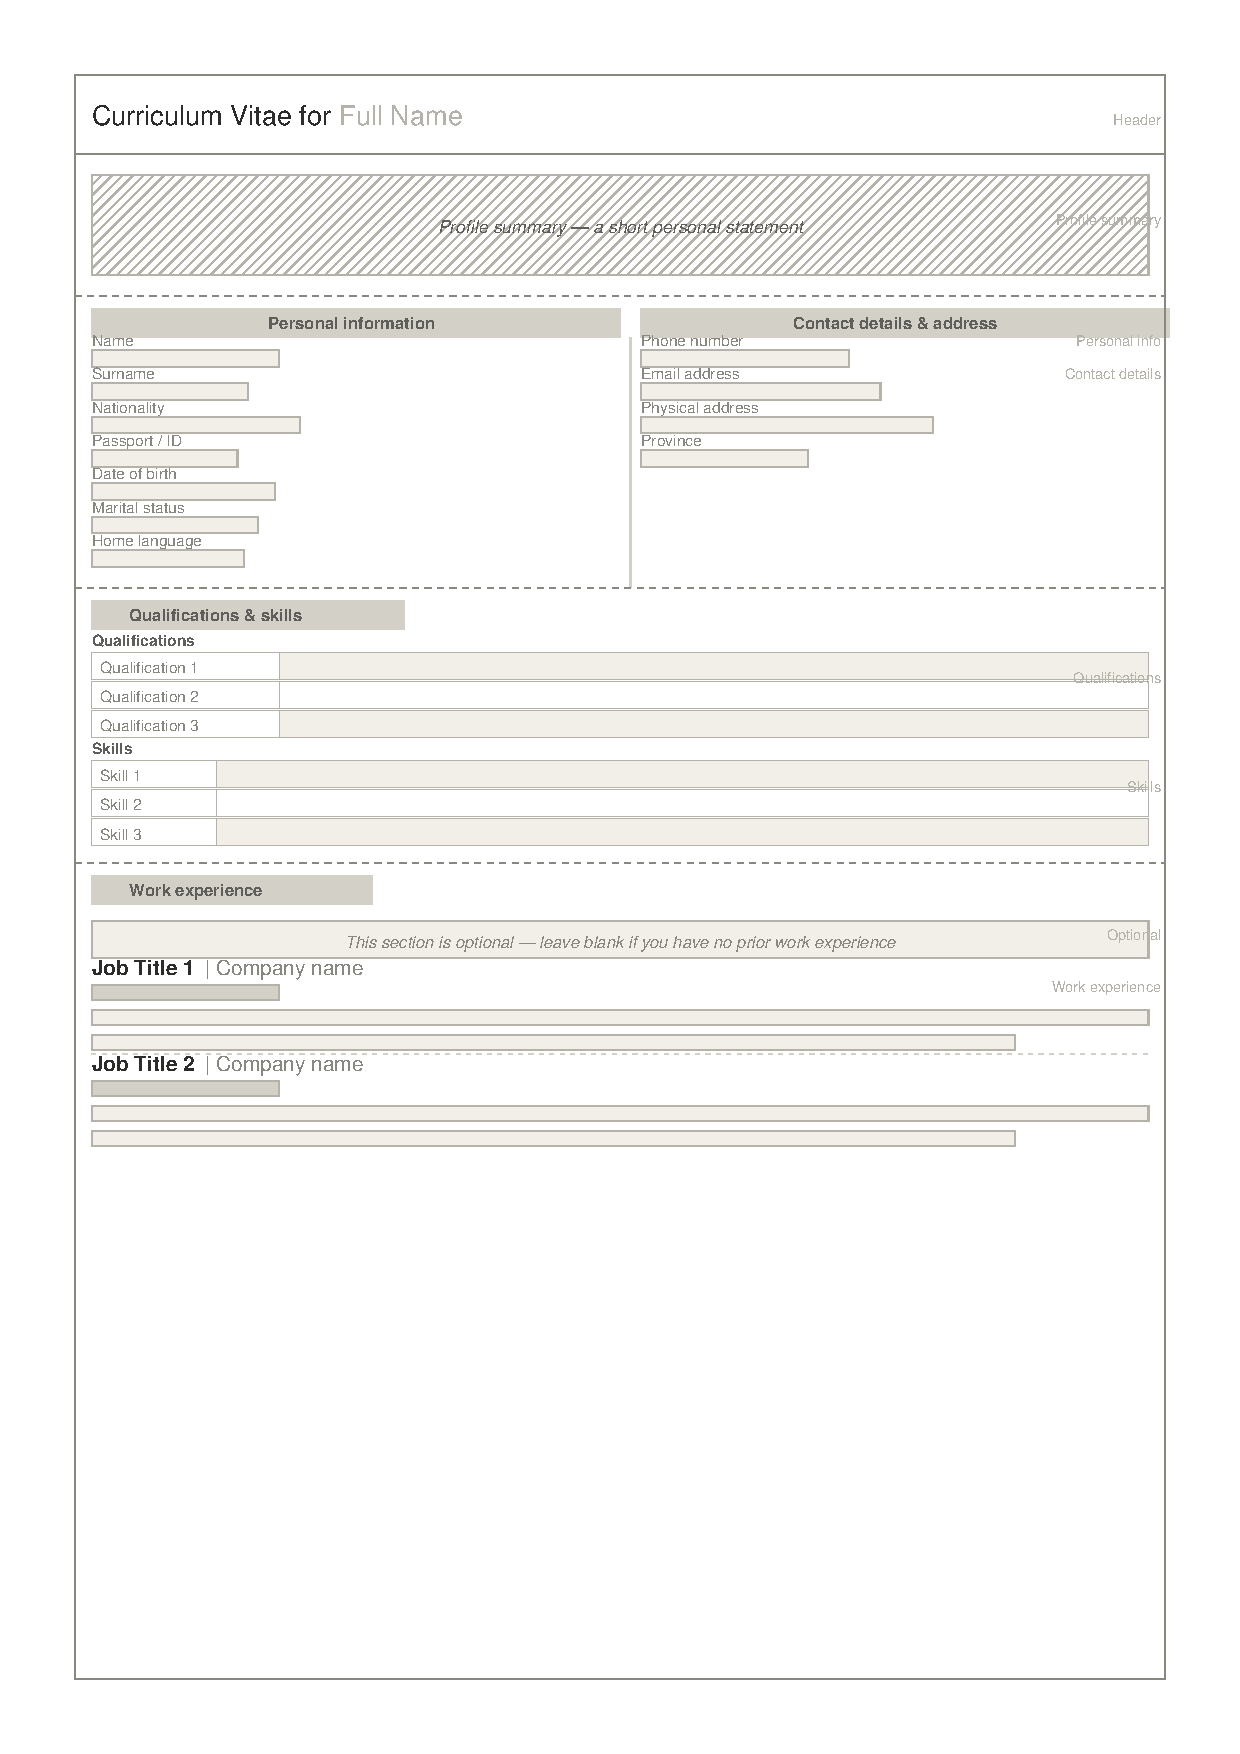
\includegraphics[width=0.75\linewidth]{dissertation/figures/CV_Wireframe.pdf}
\caption{Template CV}
\label{fig:template_cv}
\end{figure}

\FloatBarrier

\begin{figure}[H]
\centering
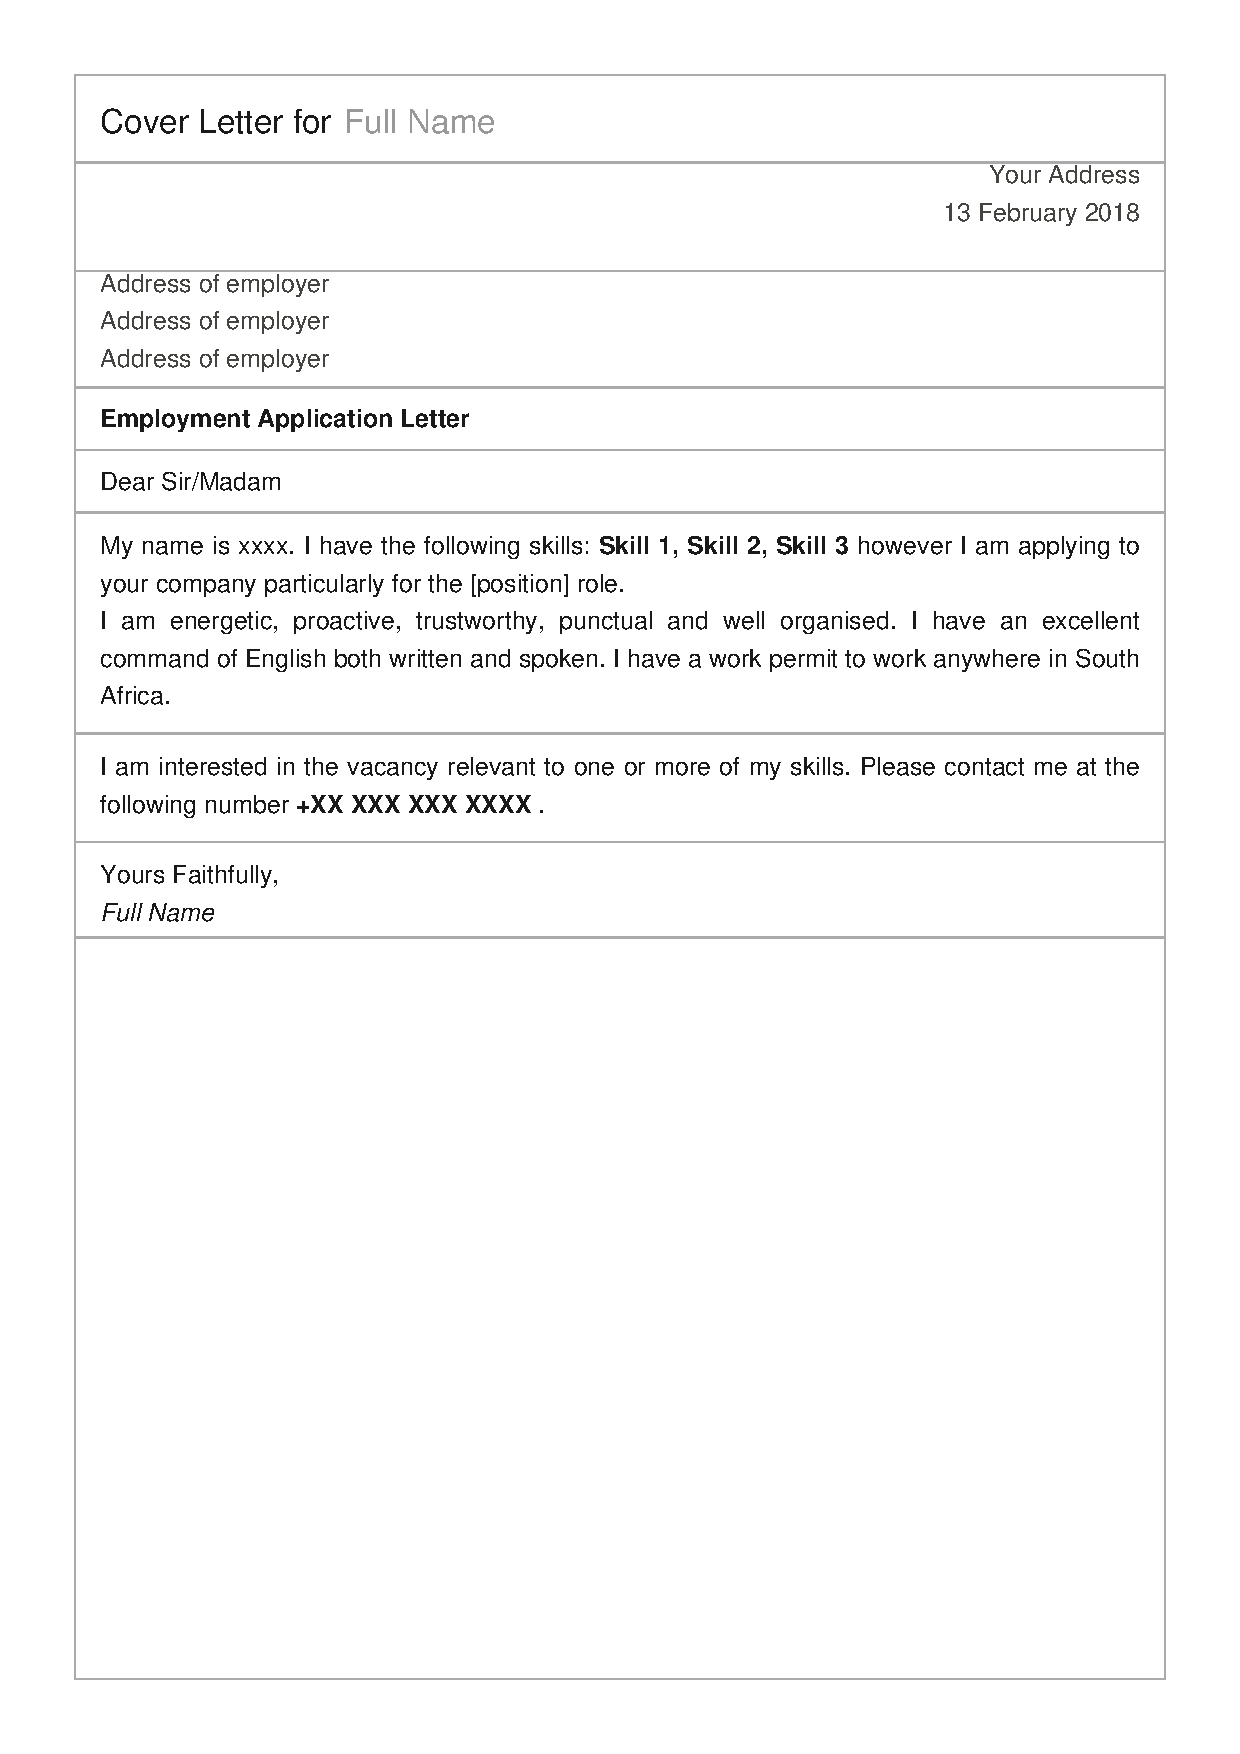
\includegraphics[width=0.75\linewidth]{dissertation/figures/Cover_Letter_Wireframe1.pdf}
\caption{Template Cover letter}
\label{fig:template_coverletter}
\end{figure}

\FloatBarrier
%------------------------------------------------
\subsection{Custom Job Notifications}

Most of the participants appreciated the daily notification system. Participant 4 stated that “emailing and SMSing were the best [features] for me. Since I am that kind of person who is always on the internet, it is very easy for me to know what is coming”. Participant 3 stated, “they give us the available jobs. Instead of going and search for yourselves”. And Participant 3 further compared the application to another, “they are different because Khanyo [Khanya job network] send you an email but Job alert give you a late job post…some of the job from job alert are the post that I don’t qualify for”.

%------------------------------------------------
\subsection{Accessing the Internet}

In cycle three, all participants indicated they use the internet. They make use of the internet through their phones, in one case using a tablet and sometimes at NGO computers. Participant 7, who was the only participant who did not have an internet enabled device stated, “I have access when I get here or when I go to Internet Café”.

%------------------------------------------------
\subsection{Custom Job Notifications}

Most of the participants appreciated the daily notification system. Participant 4 stated that “emailing and SMSing were the best for me. Since I am that kind of person who is always on the internet, it is very easy for me to know what is coming”. Participant 3 stated, “they give us the available jobs. Instead of going and search for yourselves”. And Participant 3 further compared the application to another, “they are different because Khanyo [Khanya job network] send you an email but Job alert give you a late job post… some of the job from job alert are the post that I don’t qualify for”. 
%------------------------------------------------
\subsection{Self-descriptions}

The job seekers had to describe their strengths to stand out for employment in the registration form. Table~\ref{tab:self_descriptions} lists the job seeker’s descriptions and the modifications by the researcher after data collection.

\begin{table}[H]
\centering
\caption{Job seekers’ Descriptions}
\label{tab:self_descriptions}
\renewcommand{\arraystretch}{1.2}
\begin{tabularx}{\textwidth}{
|>{\centering\arraybackslash}p{1.5cm}|
X|
X|
}
\hline
\rowcolor{gray!30}
\textbf{Job seeker} & \textbf{Own descriptions} & \textbf{Edited Description} \\
\hline

1 & im every dedicated person who can get long with poelple & I am a very dedicated person who can get along with people. \\
\hline

2 & I am a talkative person \& also a good listener. & I am a talkative person \& also a good listener. \\
\hline

3 & I m motivated and hard worker & I am a motivated person and a hard worker. \\
\hline

4 & I am hard worker and willing to take any task given to me. & I am a hard worker and willing to take any task given to me. \\
\hline

5 & I am a quick learner, I deliver on time and I work well under pressure. I have good listening skills and I am a quick learner. & I am a quick learner, I deliver on time and I work well under pressure. I have good listening skills and I am a quick learner. \\
\hline

6 & I am a hard-worker. I am willing to work. & I am a hard-worker. I am willing to work. \\
\hline

7 & i am an energetic,patient,honest man willing to learn. & I am an energetic, patient, honest man willing to learn. \\
\hline

8 & I am a hard worker, I also like to work with people to get to know and learn new things. I am a person who is willing to gain more experience. I am a benevolent person and I have a calm personality. I am willing to work at any job that requires matric. I passed my matric with a bachelor qualification. & I am a hard worker, I also like to work with people to get to know and learn new things. I am a person who is willing to gain more experience. I am a benevolent person and I have a calm personality. I am willing to work at any job that requires matric. I passed my matric with a bachelor qualification. \\
\hline

9 & I am energetic, proactive, industrious, trustworthy, punctual, sociable, team player, goal-oriented and well organized. I have an excellent command of English language both written and spoken. I have a work permit to work anywhere in South Africa. I also have ten years of teaching experience and I enjoy working with children. & I am an energetic, proactive, industrious, trustworthy, punctual, sociable, team player, goal-oriented and well organized individual. I have an excellent command of English language both written and spoken. I have a work permit to work anywhere in South Africa. I also have ten years of teaching experience and I enjoy working with children. \\
\hline

10 & I am time conscious, I a team player, I am a quick leaner. & I am time conscious, I a team player, I am a quick learner. \\
\hline

\end{tabularx}
\end{table}

\section{Discussion}

\subsection{Implications for Design for Co-design}

When we embarked on this project we had planned for it to be fully a Co-design project, however, there were limitations which affected the level of participation and design. The JR programs lasted three or four weeks and thus we could not interact with the same audience for each cycle, therefore we could not get user inputs continually beyond one cycle. We found that there was a limited chance for our users to become familiar with our Co-design methods as opposed to when participants are available for longer periods \cite{gitau2012} where users could be given an opportunity to gain exposure and learn in their own ways and at their own pace. As with many participant groups, our participants were not able to program and thus the development aspect was not directly Co-designed with the participants. Some of our participants could not speak English well and therefore struggled to express their views in English. This also limited their ability to describe their strengths for a well-marketed CV.

For equity to truly be achieved with Co-design, all participants should indicate their satisfaction on the eventual design, and in the case where there is a great imbalance between the satisfaction levels, another Co-design cycle should be embarked to adjust the design. We realized that with a design set-up such as ours this could not be achieved as there was no opportunity for all Co-designers to meet in a single sitting as students graduated from the JR classes at different times.

%------------------------------------------------
\subsection{Implications for Design for Unemployment in Africa}

Having access to jobs and one’s skills being known by potential employers are very important, however, not having sought out skills is a downside. Five of the nine participants had only matric or lower qualifications. Many jobs are only open to persons with a bachelor’s degree even when the job description does not directly need a bachelor’s degree. This is in line with statistics that indicate that individual with: tertiary qualification, Matric and less than matric have an unemployment rate of 14\%, 34\%, and 42\% respectively \cite{statssa2015}, therefore those with less than matric qualification often struggle more to find work than those with Matric level and beyond. In other cases, very specific skills are required for a specific job, often these skills are not part of the syllabus taught at matric level. For example, to be a driver requires a license certification which is not attained at matric level. Our participants listed various skills which are detailed in the findings section. In some cases, the participants had skills for which they did not have certificates to attest to the skills and thus it is challenging to find jobs with those skills. Although Participant 3 was employed as a cleaner, he was not satisfied with the job and wanted a different job. This is the case for individuals working in a role they do not qualify for, do not like or are not earning enough from.

Participant 10 made use of our application and got a job. He was employed as a general maintenance manager, which is classified as a skilled job \cite{statssa2015}, but when he got to the workplace, he was given a different job: “It was a half day title. I was changed to a wine seller”, which is either a low-skilled or a semi-skilled job \cite{statssa2015}. This could be because the participant did not have the skills required for the job he got because the participant had indicated he was a qualified English teacher and did not mention possessing any managerial qualification to take up the role of a maintenance manager. Another possibility is that the employer believed that advertising the post of a “manager” would attract people with higher skills to try to attract the highly skilled who are few in the society with statistics indicating that South Africa only had 25\% skilled workers in 2014 \cite{statssa2015}. During one of the walkthrough sessions in cycle 2, Participant 6 had indicated the system should allow individuals to list any number of skills as opposed to limiting it to a fixed number as was in the prototyped app and this recommendation is important when implementing a system for job seekers with low skills to increase their range of job matches more so as they frequently move in and out of employment.

From our finding Participant 3 indicated that Job Alert’s (a job search application) posts are “post that I don’t qualify”. Some job sites do not match the jobs to the user’s skill set. Indeed.com, for example, recommends jobs based on previous searches which means if a user searches for a job for his or her relative, Indeed.com would continue to recommend similar jobs.

When finding jobs there are cases where the job seeker does not get feedback from the potential employer as to whether the participant has been successful or not. Participant 2 narrates his difficulty when asked whether he has submitted an application, “I have tried but I don’t know what is happening. Maybe it’s me who have tried in a difficult way because when SMS have entered to my email and I click there, and they tell me to submit my CV. I have tried I’m still waiting.” There is a gap in the feedback mechanism between employers and job seekers, which can be researched in the future.

Online platforms such as Mturk, give workers an opportunity to be fairly paid for short jobs as payment for each task is visible upfront whilst the payment is done once the task is completed and approved by the employer. However, payment for tasks might be very difficult in developing regions where low-skilled unemployed sometimes do not have bank accounts. Secondly existing microwork platforms limit international micro workers, outside of UK as it requires each worker to have an address in the UK \cite{brawley2016}. Another shortcoming of the platforms is that they are not designed to have chat forums where good and bad employers and workers are highlighted as such, such sights would leave micro workers prone to cyber crimes such as phishing. Workers have to utilize external social platforms to discuss which employers have a good reputation and which do not \cite{brawley2016}. Additionally, the employers’ payment for tasks is not always well regulated. In one case a worker complained, “The survey said it would take ten minutes, but it took half an hour. The pay was poor. A dollar for ten minutes is great, a dollar for half an hour is not” \cite{brawley2016} and in other cases, the employers do not pay \cite{mtsweni2014}. But a similar system where both workers and employers are rated and monitored could potentially work well, given users have internet connected devices to access tasks and accounts to receive payments for completed tasks.

We perceive a great potential in the creation of an Uber-job app. An Uber-job app can be designed like the Uber model in terms of its payment on-service-delivery system, reputation checks, location sensitivity, and transparency. Instead of an uber-driver and uber-passenger, we would have an uber-employer and an uber-employee. The uber-job system would have to request payments for securing employment and only deduct the payment once the employee has earned a salary. Paying for a service of getting a job (and earning an income) would help a job seeker attribute more value to his/her job. And paying after service delivery, that is, after an employee (former job seeker) has earned his/her first salary, would give potential employees an opportunity to be paid before having to pay for the service, therefore an unemployed job seeker would not have to worry about where to get money at the point of employment.

The Uber-job app should be designed similarly to the Uber application having a reputation management system in place by performing regular service-delivery ratings for both the Uber-employer and the uber-employee. Therefore, both the uber-employer and uber-employee would strive to offer good services. The downside of this is that there is no job security as there is no guarantee of earning enough to make a living. Each job seeker would have to have a working PC or Smartphone and good internet connectivity for the uber-job app to work well.

And to make use of methods that do not require smart devices or connectivity, one would make use of SMS and or USSD. The shortcoming of SMS and USSD is that they are slowly becoming obsolete and are not favoured for communication because there are social media platforms such as WhatsApp and Facebook which are highly graphical and speedy for encoding and decoding messages. Although ICT enablers alone would not work to lessen the unemployment situation due to the multi-dimensional nature of the issue, lack of smartphones, lack of data, lack of money and few skills available to our blue-collar job seekers.

Having humans in a process tends to be useful and even necessary. We found that the NGOs were very useful for the wellbeing of the job seekers. Although the NGOs did not promise the job seekers jobs, in many cases they found jobs for them as other organisations would come to the NGOs in search of employees, but the NGO was often filled with many such individuals, seeking jobs. The assistance the job seekers received directly through the NGOs, for example getting a mock interview from an individual at the NGO, getting practical one-on-one training on how to use computers and search on the internet, served as valuable tools for their future job hunts, and they were equipped with soft skills that could help them to retain their jobs once they get jobs. On our side, we found that the trainers from the NGOs assisted them in getting comfortable with participating in our research. When the trainers from the NGOs introduced a session, we found that the job seekers gave more diverse input in our research. In some cases, they helped to convince the job seekers to take part in the research.

Participant 10 who had a smartphone and laptop to access the internet mentioned that: “during my off days I go to Zanokhanyo network”. This indicated that the participants did not only go to the NGO centres to find jobs, but they also go to the NGO centres to make use of the computers for internet access, even when it meant travelling to the NGO office. And because the participant owned a smartphone and a laptop, we knew that there was more to why he went to the NGO sites. Perhaps the job seekers found a sense of belonging at the NGO centres or were motivated to struggle to survive knowing that there were 100s of other individuals seeking for jobs like they were.

Although they could get online trainers and had online support groups where they would meet other job seekers, the physical presence of others was necessary. We created a test application that which we hypothesize would need human monitoring, maintenance, and support for the users if it is fully deployed. A human being would be able to pick up what improvements or perhaps new services should be added to the application, moreover, a human being would be able to give better responses to queries. A job seeker described herself: “I am a talkative person \& also a good listener”. Being talkative is a quality that would discourage more than it would motivate employers to employ, however, most intelligence systems would not find any errors in the statement as it is not grammatically incorrect. Several the CV self-descriptions were not a good representation to put the job seekers’ best foot forward.

From cycle one we found that participants do not always have transport money to find jobs. This was further affirmed by participants in cycle three.

Job seekers consider CV creation expensive at about R20 \cite{gitau2012}, this cost is mediated for our participants as they would not have to create, print or go and submit physical CVs. It also reduced the amount they would spend on data to surf the internet for jobs because the jobs were sought out for them and sent to them via SMS and they would be saved from getting bitten by dogs from looking for jobs door to door. Going door to door allowed the job seekers to search for jobs at his or her own convenience, however, it left the job seeker at the mercy of their target place.


\section{Conclusion}

Trade-offs exist between bringing the marginalized communities on par with the advantaged and yet attempting to utilize technologies that are convenient or reachable to the marginalized communities. We notice the need for humans in the scaling up of automated systems such as automated jobs notification and automated CV creation. Humans are needed for supporting automated systems or verifying the information on the systems are correct and rightly presented. When automated systems need input from users, the input process becomes a bottleneck for the automated systems. Overall, we found that the artefact was promising as all the participants wanted to use it, and in the two weeks, one had gotten a job through it. We believe that our findings after the deployment offers insights for a future designer/business to be enacted to create an implemented version of the prototyped artefact.